\documentclass[ ../main.tex]{subfiles}
%\providecommand{\mainx}{..}
\begin{document}
In what follows, we provide a theoretical implementation of the \emph{oblivious 
set} that obtains optimality in the following ways:
\begin{enumerate}
    \item The space complexity obtains the theoretical lower-bound of an approximate set with a false positive rate $\fprate$ and a false negative rate $\fnrate$.
    \item The entropy obtains the upper bound. This is necessarily the case since it obtains the optimal space complexity.
\end{enumerate}

TODO: make an absolute efficiency measure for a given entropy level. Mainly, this means the entropy of the cardinality. You can trade entropy on this for space efficiency.

\begin{definition}[Cartesian product]
Let $\Set{X}[1],\ldots,\Set{X}[n]$ denote $n$ sets. The set $\Set{X}[1] \times \cdots \times \Set{X}[n] = \left\{(x_1,\ldots,x_n) \colon x_1 \in \Set{X}[1] \land \cdots \land x_n \in \Set{X}[n]\right\}$ is called the Cartesian product of sets $\Set{X}[1],\ldots,\Set{X}[n]$.
\end{definition}
A shorthand notation for the Cartesian product $\Set{X} \times \Set{X} \times \Set{X}$ is denoted by $\Set{X}^3$.

The binary set $\{0,1\}$ is denoted by $\Set{B}$. The set of all bit (binary) strings of length $n$ is therefore $\Set{B}^n$. The cardinality of $\Set{B}^n$ is
\begin{equation}
    \Card{\Set{B}^n} = 2^n\,.
\end{equation}
The set of all bit strings of length $n$ or less is denoted by $\Set{B}^{\leq n}$, which has a cardinality $2^{n+1}-1$. The countably infinite set of all bit strings, $\Set{B}^{\leq \infty}$, is also denoted by $\Set{B}^{*}$.

The bit length of an object $x$ is denoted by
\begin{equation}
    \BL(x)\,,
\end{equation}
e.g., the bit length of any $x \in \Set{B}[n]$ is $\BL(x) = n$.

A (convenient) one-to-one correspondence between $\Set{B}$ and $\NatSet$ is given by the following definition.
\begin{definition}
\label{def:mapping}
Let the set of bit strings $\Set{B}$ and the set of natural numbers $\NatSet$ have the bijection given by
\begin{equation}
    (b_1 \, b_2 \, \cdots \, b_m) \longleftrightarrow 2^m + \sum_{j=1}^{m} 2^{m - j} b_j\,.
\end{equation}
We denote the mapping of a bit string (or natural number) $x$ by $x'$.
\end{definition}
An important observation of this mapping is that a natural number $n$ maps to a bit string $n'$ of length $\BL(n') = \lfloor \log_2 n \rfloor$.
\begin{example}
Consider the number $100$ (base $10$). To determine the bit string $100'$, we perform the following steps:
\begin{enumerate}
    \item The length of $100'$ is $\lfloor \log_2 100 \rfloor = 6$.
    \item Subtract $2^6 = 64$ from $100$ which results in $36$.
    \item $36_{10}$ in binary is $100100_2$.
    \item $100' = (1\,0\,0\,1\,0\,0)$.
\end{enumerate}
\end{example}

A \emph{hash function} is related to countable sets $\Set{B}$ and $\Set{B}[n]$ and is given by the following definition.
\begin{definition}
A \emph{hash function} $\hash \colon \Set{B} \mapsto \Set{B}^n$ is a function such that all bit strings of arbitrary-length are mapped (hashed) to bit strings of fixed-length $n$. For a given $x \in \Set{B}$, $y = \hash(x)$ is denoted the \emph{hash} of $x$.
\end{definition}

The \gls{gls-shs} is a data type that implements the \emph{oblivious set} 
abstract data type. The implementation consists of a product data structure 
(tuple) $\Set{B}^k \times \Set{B}^{*}$, an algorithm that \emph{generates} the 
data structure, and an algorithm that implements the \emph{member-of} function 
by \emph{querying} the data structure. 

The \gls{gls-shs} assumes that random oracles are available.
\begin{definition}
\label{def:randomoracle}
A random oracle, denoted by $\ro \colon \Set{B}^\infty \mapsto \Set{B}^\infty$, is a theoretical \emph{hash function} whose output is uniformly distributed over the elements of $\Set{B}^\infty$.
\end{definition}

The implementation of the algorithm that generates the data structure for the \gls{gls-shs} that implements an \emph{approximate} \emph{oblivious set} is given by the following theorem.
\begin{theorem}[\Gls*{gls-shs}]
The data structure generated by
\begin{equation}
    \OASet \gets \MakeApproxSet(\Set{S},\fprate)
\end{equation}
as given by \cref{alg:makeset} is an \emph{oblivous set} of $\Set{S} \subset \Set{U}$ with a \emph{\gls{gls-fprate}} $\fprate \in \left\{2^{-k} \colon k \in \NatSet\right\}$ and a \emph{false negative rate} $\fnrate \in \left\{\frac{j}{m} \colon j \in \{1,\ldots,m\}\right\}$.
\end{theorem}
\begin{proof}
In order for the \gls{gls-shs} to be an \emph{oblivious set} of $\OASet{S}$, it must also be an \emph{approximate set}. Two be an approximate set of $\Set{S}$, it must satisfy the two conditions given by \cref{def:approx_set}:
\begin{enumerate}
    \item $\Set{S}$ is a subset of $\OASet{S}$. This condition guarantees that no \emph{false negatives} may occur.
    \item An element in $\Set{B}$ that is not a member of $\Set{S}$ is a member of $\OASet{S}$ with a probability $\fprate$, denoted the \gls{gls-fprate}, i.e.,
    \begin{equation}
        \Prob{\RV{X} \in \OASet{S} \given \RV{X} \notin \Set{S}} = \fprate\,.
    \end{equation}
\end{enumerate}
%If an element $x \in \Set{U}$ is a member of $\Set{S}$, \Contains{$\PASet{S}$,$x$} returns \True and otherwise returns %\False with probability $\fprate$ and \True with probability $1-\fprate$. We denote this data structure %the \gls{gls-shs}.

To prove the first condition, note that \cref{alg:contains} tests any element $x$ for membership in $\PASet{S}$ by computing the hash of $x$ concatenated with the bit string $b_n$ and returning \True if the hash is $h_k$ where \cref{alg:makeset} finds bit strings $b_n$ and $h_k$ such that each element of $\Set{S}$ concatenated with $b_n$ hashes to $h_k$.

To prove the second condition, suppose we have a set $\Set{S} = \{x_1,\ldots,x_m\}$ and each element in $\Set{S}$ hashes to $y = \hash(x_1)$. By \cref{asm:ro_approx}, $\hash \colon \Set{B}^* \mapsto \Set{B}^k$ approximates a random oracle and thus uniformly distributes over its domain of $2^k$ possibilities. Since $y$ is a particular element in $\Set{B}^k$, the probability that an element not in $\Set{S}$ hashes to $y$ is $2^{-k}$.
\end{proof}

\begin{algorithm}
    \caption{Implementation of \protect\MakeApproxSet over a finite universe $\Set{U}$}
    \label{alg:makeexactobset}
    \DontPrintSemicolon
    \SetKwProg{func}{function}{}{}
    \KwIn
    {
        $\Set{S}$ is a subset of a finite universal set $\Set{U}$.
    }
    \KwOut
    {
        An \emph{oblivious} exact set of $\Set{S}$.
    }
    \func{\MakeApproxSet{$\Set{S}$, $\fprate$, $\fnrate$}}
    {
        $\Set{S}_{\Set{B}} \gets \left\{\Encode_{\Set{U} \mapsto \Set{B}}(x) \colon x \in \Set{S}\right\}$\;
        $\Set{\overline{S}}_{\Set{B}} \gets \left\{\Encode_{\Set{U} \mapsto \Set{B}}(x) \colon x \in \Set{\overline{S}}\right\}$\;        
        \tcp{To find the smallest bit string, search for a bit string of length $n$ in ascending order.}
        \For{$n \gets 0$ \KwTo $\infty$}
        {
            \For{$j \gets 1$ \KwTo $2^n$}
            {
                $\found \gets \True$\;
                \tcp{To maximize \emph{entropy} we try bit strings of length $n$ in random order.}
                $b_n \gets $ a bit string of length $n$ randomly drawn from $\Set{B}[n]$ without replacement\;
                $h_k \gets \Null$\;
                \For{$x \in \Set{S}_{\Set{B}}$}
                {
                    \If{$h_k = \Null$}
                    {
                        $h_k \gets \hash\!\left(x \catop b_n\right) \mod (k+1)$\;
                    }
                    \ElseIf{$h \neq \hash\!\left(x \catop b_n\right) \mod (k+1)$} 
                    {
                        $\found \gets \False$\;
                    }
                }
                \For{$x \in \Set{\overline{S}}_{\Set{B}}$}
                {
                    \If{$h = \hash\!\left(x \catop b_n\right) \mod (k+1)$} 
                    {
                        $\found \gets \False$\;
                    }
                }
                \If{\found}
                {
                    \tcp{This tuple is the data structure of the \gls{gls-shs}.}
                    \Return $(h_k, b_n)$\;
                }
            }
        }
    }
\end{algorithm}



Condition for maxium entropy:

The countably infinite intersection of separate instances of an approximate oblivious set of $\Set{S}$ where $\fnrate > 0$ is the empty set,
\begin{equation}
    \bigcap_{j} \OASet{S}[j] = \EmptySet\,,
\end{equation}
where $\OASet{S}[1],\OASet{S}[2],\ldots$ are random instances of an approximate oblivious set of $\Set{S}$.

TODO: this directly follows from the sampling distribution and taking the limit.

In the case of a positive approximate oblivious set, where $\fnrate = 0$, the countably infinite intersection of separate instances of a positive approximate oblivious set of $\Set{S}$ is $\Set{S}$,
\begin{equation}
    \bigcap_{j} \OPASet{S}[j] = \Set{S}\,.
\end{equation}

A countable union of separate instances of a negative approximate oblivious set of $\Set{S}$ is the complement of $\Set{S}$
\begin{equation}
    \bigcap_{j} \ONASet{S}[j] = \Set{\SetComplement[S]}\,.
\end{equation}



Exact oblivious set:
\begin{equation}
    k (\rho u - 1) + (u \log_2(1 - 2^{-k})(\rho - 1)
\end{equation}

\begin{equation}
    k (\rho u - 1)/m + (u \log_2(1 - 2^{-k})(\rho - 1)/m
\end{equation}

\begin{equation}
    k\left(1 - \frac{1}{u \rho}\right) + \log_2\!\left(1 - 2^{-k}\right)\left(1 - \frac{1}{\rho}\right)
\end{equation}

\begin{equation}
    k (\rho - \frac{1}{u}) + \log_2(1 - 2^{-k}(\rho - 1) \; \si{bits \per element in universal set}
\end{equation}


\begin{theorem}
\begin{equation}
    \min_k k (\rho - \frac{1}{u}) + \log_2(1 - 2^{-k}(\rho - 1) \; \si{bits \per element in universal set}
\end{equation}
\end{theorem}



The above algortihm for generating exact oblivious sets has a space complexity of $u$ bits. Assuming $m$ is not too much smaller than $u$, i.e., $\Set{S}$ is dense, this is the theoretical lower-bound for sets over finite universes.

If $m$ is not dense, then trying larger singular hash lengths will result in a better lower-bound.

Suppose you are interested in creating exact oblivious sets over the universe of bit strings up to length $n$, denoted by $\Set{B}[\leq n]$. Then, there are $\Card{\Set{B}[\leq n]} = 2^{n+1} - 1$ bit strings in the universe. In this case, the set has a lower-bound given by
$\mathcal{O}(n)$.

\begin{algorithm}
    \caption{Implementation of \protect\MakeApproxSet}
    \label{alg:makeset}
    \DontPrintSemicolon
    \SetKwProg{func}{function}{}{}
    \KwIn
    {
        $\Set{S}$ is finite subset of a universal set $\Set{U}$, $\fprate$ is the false positive rate, and $\fnrate$ is the maximum false negative rate.
    }
    \KwOut
    {
        An \emph{oblivious, approximate set} $\Set{S}^*$.
    }
    \func{\MakeApproxSet{$\Set{S}$, $\fprate$, $\fnrate$}}
    {
        $\Set{S}_{\Set{B}} \gets \left\{\Encode_{\Set{U} \mapsto \Set{B}}(x) \colon x \in \Set{S}\right\}$\;
        \tcp{$p$ is the minimum number of elements in $\Set{S}$ that must be true positives.}
        $p \gets (1 - \fnrate) \Card{\Set{S}}$\;
        \tcp{A random oracle that hashes to $k$ bits has a probability $\fprate = 2^{-k}$ of hashing to a particular value.}
        $k \gets -\log_2 \fprate$\;
        \tcp{To find the smallest bit string, search for a bit string of length $n$ in ascending order.}
        \For{$n \gets 0$ \KwTo $\infty$}
        {
            \For{$j \gets 1$ \KwTo $2^n$}
            {
                $\found \gets \True$\;
                \tcp{To maximize \emph{entropy} we try bit strings of length $n$ in random order.}
                $b_n \gets $ a bit string of length $n$ randomly drawn from $\Set{B}[n]$ without replacement\;
                \tcp{A minimum of $p$ elements must have the same hash.}
                $\Set{M} \gets \text{all subsets of $p$ elements from $\Set{S}$}$\;
                \For{$\Set{P} \in \Set{M}$}
                {
                    \tcp{Let the $p$ elements in $\Set{P}$ be denoted
                    by $x^{(1)},\ldots,x^{(p)}$.}
                    $h_k \gets \hash\!\left(x^{(1)} \catop b_n\right) \mod k$\;
                    \For{$i \gets 2$ \KwTo $p$}
                    {
                        \If{$h_k \neq \hash\!\left(x^{(j)} \catop b_n\right) \mod k$} 
                        {
                            $\found \gets \False$\;
                        }
                    }
                }
                \If{\found}
                {
                    \tcp{This tuple is sufficient to code the \gls{gls-shs}.}
                    \Return $(h_k, b_n)$\;
                }
            }
        }
    }
\end{algorithm}















\begin{algorithm}
    \caption{Implementation of \protect\MakeApproxSet}
    \label{alg:makeset}
    \DontPrintSemicolon
    \SetKwProg{func}{function}{}{}
    \KwIn
    {
        $\Set{S}$ is a \emph{finite} \gls{gls-set} over $\Set{U}$, $\fprate \in \left\{2^{-k} \colon k \in \NatSet \cup \{ 0 \}\right\}$ is the false positive rate, and $\fnrate \in \left\{j / \Card{\Set{S}} \colon j = 1,\ldots,\Card{\Set{S}}\right\}$ is the false negative rate.
    }
    \KwOut
    {
        An approximate \emph{oblivious set} $\OASet{S}$.
    }
    \func{\MakeApproxSet{$\Set{S}$, $\fprate$, $\fnrate$}}
    {
        $\Set{S}_{\Set{B}} \gets \left\{\Encode_{\Set{U} \mapsto \Set{B}}(x) \colon x \in \Set{S}\right\}$\;
        \tcp{$p$ is the number of elements in $\Set{S}$ that must be false negatives.}
        $p \gets (1-\fnrate) \Card{\Set{S}}$\;
        \tcp{A random oracle that hashes to $k$ bits has a probability $\fprate = 2^{-k}$ of hashing to a particular value.}
        $k \gets -\log_2 \fprate$\;
        \tcp{To find the smallest bit string, search for a bit string of length $n$ in ascending order of length.}
        \For{$n \gets 0$ \KwTo $\infty$}
        {
            \For{$j \gets 1$ \KwTo $2^n$}
            {
                \tcp{To maximize \emph{entropy} we try bit strings of length $n$ in random order.}
                $b_n \gets $ a bit string randomly drawn from $\Set{B}[n]$ without replacement\;
                $h(x) \over{\text{def}}{=} \hash\!\left(x \catop b_n\right) \mod k$ for $x \in \Set{S}$\;
                
                \If{$\Card{\Set{X}} = p$}
                {
                    \tcp{This tuple is sufficient to code the \gls{gls-shs}.}
                    \Return $(h_k, b_n)$\;
                }
            }
        }
    }
\end{algorithm}













\begin{algorithm}
    \caption{Implementation of \protect\Contains}
    \label{alg:contains}
    \DontPrintSemicolon
    \KwIn
    {
        $\PASet{S}$ is the \gls{gls-shs} to query and $x$ is the element to test for membership.
    }
    \KwOut
    {
        \True if $x \in \PASet{S}$ otherwise \False. If we rephrase this with respect to $\Set{S} \subset \PASet{S}$, then \True if $x \in \Set{S}$ and otherwise \True with probability $\fprate$ and \False with probability $1 - \fprate$, where $\fprate$ is the false positive rate of $\PASet{S}$.
    }
    \SetKwProg{func}{function}{}{}    
    \func{\Contains{$\PASet{S}$,$x$}}
    {
        \tcp{The \gls{gls-shs} $\PASet{S}$ is coded by the tuple $(b_n, h_k)$, where $b_n$ is a bit string of length $n$ and $h_k$ is the singular hash.}
        $k = \BL(h_k)$\;
        \uIf{\hash{$x \catop b_n$}$\mod k = h_k$}
        {
            \tcp{False positives occur with probability $\fprate = 2^{-k}$.}
            \Return \True\;
        }
        \uElse
        {
            \Return \False\;
        }
    }
\end{algorithm}

\begin{figure}
    \centering
    %% Creator: Inkscape inkscape 0.92.1, www.inkscape.org
%% PDF/EPS/PS + LaTeX output extension by Johan Engelen, 2010
%% Accompanies image file 'shs.pdf' (pdf, eps, ps)
%%
%% To include the image in your LaTeX document, write
%%   \input{<filename>.tex}
%%  instead of
%%   \includegraphics{<filename>.pdf}
%% To scale the image, write
%%   \def\svgwidth{<desired width>}
%%   \input{<filename>.pdf_tex}
%%  instead of
%%   \includegraphics[width=<desired width>]{<filename>.pdf}
%%
%% Images with a different path to the parent latex file can
%% be accessed with the `import' package (which may need to be
%% installed) using
%%   \usepackage{import}
%% in the preamble, and then including the image with
%%   \import{<path to file>}{<filename>.pdf_tex}
%% Alternatively, one can specify
%%   \graphicspath{{<path to file>/}}
%% 
%% For more information, please see info/svg-inkscape on CTAN:
%%   http://tug.ctan.org/tex-archive/info/svg-inkscape
%%
\begingroup%
  \makeatletter%
  \providecommand\color[2][]{%
    \errmessage{(Inkscape) Color is used for the text in Inkscape, but the package 'color.sty' is not loaded}%
    \renewcommand\color[2][]{}%
  }%
  \providecommand\transparent[1]{%
    \errmessage{(Inkscape) Transparency is used (non-zero) for the text in Inkscape, but the package 'transparent.sty' is not loaded}%
    \renewcommand\transparent[1]{}%
  }%
  \providecommand\hashtatebox[2]{#2}%
  \ifx\svgwidth\undefined%
    \setlength{\unitlength}{214.63718569bp}%
    \ifx\svgscale\undefined%
      \relax%
    \else%
      \setlength{\unitlength}{\unitlength * \real{\svgscale}}%
    \fi%
  \else%
    \setlength{\unitlength}{\svgwidth}%
  \fi%
  \global\let\svgwidth\undefined%
  \global\let\svgscale\undefined%
  \makeatother%
  \begin{picture}(1,0.55063496)%
    \put(0.38,0.078){\color[rgb]{0,0,0}\makebox(0,0)[lb]{\smash{$\mathsmaller{\hash\left(x_2 \cat b\right) \mod 4}$}}}%
    \put(0.08843285,0.51926543){\color[rgb]{0,0,0}\makebox(0,0)[lb]{\smash{set $\Set{S}$}}}%
    \put(0,0){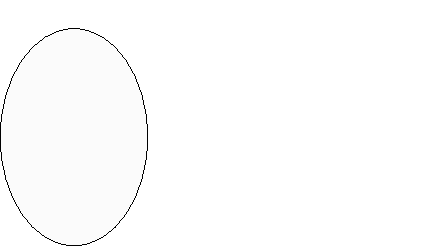
\includegraphics[width=\unitlength,page=1]{fig_shs.pdf}}%
    \put(0.09242613,0.24054801){\color[rgb]{0,0,0}\makebox(0,0)[lb]{\smash{$x_1$}}}%
    \put(0.12846631,0.36240699){\color[rgb]{0,0,0}\makebox(0,0)[lb]{\smash{$x_3$}}}%
    \put(0.13833525,0.11371431){\color[rgb]{0,0,0}\makebox(0,0)[lb]{\smash{$x_2$}}}%
    \put(0.92073981,0.50635972){\color[rgb]{0,0,0}\makebox(0,0)[lt]{\begin{minipage}{0.53112884\unitlength}\raggedright \end{minipage}}}%
    \put(0,0){\includegraphics[width=\unitlength,page=2]{fig_shs.pdf}}%
    \put(0.41093171,0.41327568){\color[rgb]{0,0,0}\makebox(0,0)[lb]{\smash{$\mathsmaller{\hash\left(x_3 \cat b\right) \mod 4}$}}}%
    \put(0.35,0.275){\color[rgb]{0,0,0}\makebox(0,0)[lb]{\smash{$\mathsmaller{\hash\left(x_1 \cat b\right) \mod 4}$}}}%
    \put(0,0){\includegraphics[width=\unitlength,page=3]{fig_shs.pdf}}%
    \put(0.81940596,0.29320931){\color[rgb]{0,0,0}\makebox(0,0)[lb]{\smash{$0\,1\,0\,0$}}}%
    \put(0.76349761,0.2128412){\color[rgb]{0,0,0}\makebox(0,0)[lb]{\smash{$\fprate = 2^{-4}$}}}%
  \end{picture}%
\endgroup%

    \caption{\emph{Singular Hash Set} over a \emph{countably infinite} universe}
    \label{fig:my_label}
\end{figure}

\subsection{Space complexity}
The probability that every element of $\Set{S}$ collides for a particular bit string in \cref{alg:ph} is given by the following theorem.
\begin{theorem}
The probability that a bit string $b \in \Set{B}$ results in perfect collision in \cref{alg:ph} is given by
\begin{equation}
\label{eq:p_m_N}
    \fprate^{m-1}\,,
\end{equation}
where $m = \Card{\Set{S}}$ and $\fprate$ is the specified false positive rate.
\end{theorem}
\begin{proof}
Suppose we have a set $\Set{S} = \{x_1,\ldots,x_m\}$ and $x_1$ hashes to $y = \hash_{\Set{S}}(x_1)$, where $\hash_{\Set{S}} \colon \Set{B}^{*} \mapsto \Set{B}^k$ is a random hash function that uniformly distributes over its domain of $2^k$ possibilities. Since $y$ is a particular element in $\Set{B}^k$, the probability that $x_j$ for $j=2,\ldots,m$ hashes to $y$ is given by
\begin{equation}
    \frac{1}{2^k} = \fprate\,.
\end{equation}
Since $\hash_{\Set{S}}$ is a random hash function, the hashes of $x_1,\ldots,x_m$ are independent. Thus, the joint probability that $x_2, \ldots, x_m$ hash to $y$ is given by the product of their marginal probabilities
\begin{equation}
    \fprate^{m-1}\,.
\end{equation}
\end{proof}

\begin{theorem}
The expected bit length of the Singular Hash Set obtains the information-theoretic lower-bound given by
\begin{equation}
    -\log_2 \fprate \; \si{bits \per element}\,,
\end{equation}
where $\fprate$ is the false positive rate.
\end{theorem}
\begin{proof}
The space required for the \gls{gls-shs} found by \cref{alg:makeset} is of the order of the length $n$ of the bit string $b_n$. Therefore, for space efficiency, the algorithm exhaustively searches for a bit string in the order of increasing size $n$.

We are interested in the first case when a perfect collision occurs, which is a geometric distribution with probability of success $\fprate^{m-1}$ as given by the discrete random variable
\begin{equation}
    \RV{Q} \sim \geodist \!\left(\fprate^{m-1}\right)\,.
\end{equation}
By \cref{def:mapping}, the \nth trial uniquely maps to a bit string of length $m = \lfloor \log_2 n \rfloor$. Thus, the bit string is a random length given approximately by
\begin{equation}
    \RV{N} = \log_2 \RV{Q} \; \si{bits}\,.
\end{equation}
This is a slight \emph{overestimate} since we are simplifying by avoiding the floor function.

We approximate the logarithm with a second-order Taylor series around the \emph{expected} value of $\RV{Q}$ as given by
\begin{equation}
    \RV{N} \approx
        \log_2 \Expect{\RV{Q}} -
        \frac{\log_2 e}{\Expect{\RV{Q}}}
        \left(\RV{Q} - \Expect{\RV{Q}}\right)^2 \; \si{bits}\,.
\end{equation}
We are interested in the \emph{expected} value of $\RV{N}$,
\begin{equation}
\label{eq:proofspaceexplb}
    \Expect{\RV{N}} \approx
        \log_2 \Expect{\RV{Q}} -
        \frac{\log_2 e}{\Expect{\RV{Q}}}
        \Expect{\RV{Q} - \Expect{\RV{Q}}}^2 \; \si{bits}\,.
\end{equation}
The variance of $\RV{Q}$ is given by
\begin{equation}
    \Var{\RV{Q}} = \Expect{\RV{Q} - \Expect{\RV{Q}}}^2\,,
\end{equation}
and thus we may rewrite \cref{eq:proofspaceexplb} as
\begin{equation}
\label{eq:proofspaceexplb2}
    \Expect{\RV{N}} \approx
        \log_2 \Expect{\RV{Q}} -
        \frac{\log_2 e}{\Expect{\RV{Q}}}
        \Var{\RV{Q}} \; \si{bits}\,.
\end{equation}
Since $\RV{Q}$ is geometrically distributed with a probability of success $\fprate^{m-1}$, the expectation and variance of $\RV{Q}$ is known to be
\begin{equation}
    \Expect{\RV{Q}} = \fprate^{-(m-1)}
\end{equation}
and 
\begin{equation}
    \Var{\RV{Q}} = \frac{1 - \fprate^{m-1}}{\left(\fprate^{m-1}\right)^2}\,.
\end{equation}
Plugging these values into \cref{eq:proofspaceexplb2} yields
\begin{align}
    \Expect{\RV{N}}
        &\approx \log_2 \fprate^{-(m-1)} - \frac{\log_2 e}{\fprate^{-(m-1)}} \frac{1 - \fprate^{(m-1)}}{\left(\fprate^{m-1}\right)^2}\\
        &= -(m-1) \log_2 \fprate + \left(1 - \fprate^{-(m-1)}\right) \log_2 e \; \si{bits}\,.
\end{align}
We are interested in the bits per element. There are $m$ elements, so dividing by $m$ results in
\begin{equation}
    -\frac{m-1}{m} \log_2 \fprate + \frac{1 - \fprate^{-(m-1)}}{m} \; \si{bits \per element}\,.
\end{equation}
Asymptotically, as $m \to \infty$, the expected bits per element goes to
\begin{equation}
    -\log_2 \fprate\,.
\end{equation}
\end{proof}

By \cref{eq:exp_trials}, \cref{alg:ph} has an expected time complexity that grows exponentially as $m$ grows The algorithm is intended to illustrate theoretical properties, not necessarily be used in practice.

\subsection{Entropy}

\begin{proof}
\begin{equation}
    \Entropy{\RV{N}} = -\Expect{\log_2 \PDF{\RV{N}}[\RV{N}]}\,.
\end{equation}

% pmf = \left(q^{2^n-1}\left(1-q^{2^n}\right)
\begin{align}
    \Entropy{\RV{N}}
        &= -\sum_{n=0}^{\infty} \log_2 \PDF{n}[\RV{N}] \PDF{n}[\RV{N}]\\
        &= -\sum_{n=0}^{\infty} \log_2\! \left(q^{2^n-1}\left(1-q^{2^n}\right)\right) \PDF{n}[\RV{N}]\,.
\end{align}
\begin{equation}
\begin{split}
    \Entropy{\RV{N}}
        =&-\log_2 q \sum_{n=0}^{\infty}
            (2^n-1) \PDF{n}[\RV{N}] -\\
         &\sum_{n=0}^{\infty} \log_2\left(1-q^{2^n}\right) \PDF{n}[\RV{N}]\,.
\end{split}
\end{equation}


\begin{equation}
\begin{split}
    \Entropy{\RV{N}}
        =&-\log_2 q \left[\sum_{n=0}^{\infty}
            (2^n \PDF{n}[\RV{N}]\right] -\\
         &\sum_{n=0}^{\infty} \log_2\left(1-q^{2^n}\right) \PDF{n}[\RV{N}]\,.
\end{split}
\end{equation}

\end{proof}


\begin{theorem}
The random bit string that codes the \gls{gls-shs} is a \emph{maximum entropy} coder for the \emph{approximate set} abstract data type.
\end{theorem}
\begin{proof}
The result immediately follows from the fact that the bit string is \emph{incompressible}, and thus obtains maximum entropy. The hash $h_k$ is the result of a random oracle and is thus uniformly distributed and, given that a bit string of length $n$ is found, the probability that a particular $b_n$ is found is uniformly distributed also. The only part of this that does not obtain maximum entropy is the particular bit length $n$ of $b_n$.
\end{proof}

The only information contained in the encoding of the approximate set is given by the probability mass function of the random bit length $\RV{N}$, which is a function of the cardinality of the \gls{gls-finiteset} being approximated and the false positive rate $\fprate$.

Given a set $\Set{S}$, the random bit length $\RV{N}$ of bit string $b_n$ has a probability mass concentrated around the theoretical lower-bound. Therefore, a \emph{method-of-moments} estimator of the cardinality of the set $\Set{S}$ is given by
\begin{equation}
    \hat{\Card{\Set{S}}} = -\frac{\BL\!\left(\PASet{S}\right)}{\log_2 \fprate}\,,
\end{equation}
were $\BL$ is the bit length function and $\fprate$ is the \emph{\gls{gls-fprate}}.

We may trade space complexity for entropy if desired. For instance, if the policy is to search for a bit string of a length $t$ much larger than the expected bit length, $-m \log_2 \fprate$, then
\begin{equation}
    m < -\frac{t}{\log_2 \fprate}\,.
\end{equation}
Thus, an estimator of the upper-bound on the cardinality is given by
\begin{equation}
    \hat{m}_{\rm{max}} \approx -\frac{t}{\log_2 \fprate}
\end{equation}
and an estimate of the \emph{lower-bound} is $0$ (the empty set) where the cardinality is uniformly distributed (maximum entropy) between $0$ and $\hat{m}_{\rm{max}}$, which has an entropy given by
\begin{equation}
    \log_2(1+\hat{m}_{\rm{max}})\,.
\end{equation}

The absolute space efficiency is now given by
\begin{equation}
    \frac{m}{\hat{m}_{\rm{max}}}\,,
\end{equation}
which is the \emph{maximum} efficiency possible for an approximate set with a cardinality uniformly distributed between $0$ and $\hat{m}_{\RV{max}}$.

\begin{example}
Suppose $t = r m, r > 1$, then
\begin{equation}
    \hat{m}_{\rm{max}} \approx -\frac{r m}{\log_2 \fprate}
\end{equation}
which has an entropy given by
\begin{equation}
    \log_2\!\left(1 -\frac{r m}{\log_2 \fprate}\right) \approx \log_2 r + \log_2 m + \log_2 \frac{1}{\fprate}
\end{equation}
and an absolute space efficiency $r$.
\end{example}
\end{document}